% ============================================================================
% DRAFT replacement/augmentation for main.tex section 4.1 "Monolithic (TD-MPC2/SimNorm)".
% Status: for review, NOT yet spliced. Numbers from evidence/dmc_glass_vs_tdmpc2.json (n=3
% both algos; seed-4 in flight will tighten CIs further -> live page authoritative).
% NOTE: this version corrects an n=2 over-read: at n=3 there is NO systematic return
% difference and NO systematic stability difference (both algos have collapsing seeds);
% the only robust effect is the 1.35x wall-clock cost. That is the strongest null.
% ============================================================================

\subsection{Monolithic (TD-MPC2 / SimNorm): a matched, multi-seed benchmark}
\label{sec:benchmark}

The strongest single piece of evidence for representation-abstraction redundancy is a
matched-protocol benchmark of the explicit structural-entropy (SE) abstraction
(\emph{tdmpc-glass}) against the identical monolith (\emph{tdmpc2}) --- same code,
hyperparameters, and harness, the SE objective the only changed variable --- across
\textbf{16 DMControl tasks at 1M environment steps}, with \textbf{mean $\pm$ 95\% CI over $n{=}4$
seeds} and a \textbf{wall-clock} axis (Table~\ref{tab:bench}). This upgrades the single-run levers
of \S\ref{sec:campaign} to a controlled multi-seed comparison.

\begin{table}[t]
\centering\small
\caption{DMControl return at 1M steps, tdmpc-glass (SE abstraction) vs.\ tdmpc2 (monolith),
mean$\pm$95\%CI ($n{=}4$), and per-run wall-clock. No systematic return difference (ties within CI
on 15/16; the single CI-separated case favors the monolith and tracks a collapsed glass seed); the only
robust effect is $\sim$1.35$\times$ wall-clock. Source: \texttt{evidence/dmc\_glass\_vs\_tdmpc2.json}.}
\label{tab:bench}
\begin{tabular}{lrrl}
\toprule
task & tdmpc-glass & tdmpc2 & note \\
\midrule
WalkerWalk      & $919{\pm}80$  & $971{\pm}12$  & tie \\
WalkerStand     & $969{\pm}14$  & $979{\pm}16$  & tie \\
WalkerRun       & $662{\pm}8$   & $652{\pm}34$  & tie \\
CartpoleBalance & $972{\pm}9$   & $945{\pm}50$  & tie \\
CartpoleSwingup & $836{\pm}12$  & $823{\pm}35$  & tie \\
FingerSpin      & $969{\pm}12$  & $950{\pm}32$  & tie \\
FingerTurnEasy  & $874{\pm}96$  & $920{\pm}84$  & tie \\
FingerTurnHard  & $725{\pm}155$ & $869{\pm}167$ & tie (both noisy) \\
AcrobotSwingup  & $296{\pm}11$  & $324{\pm}99$  & tie \\
HopperHop       & $196{\pm}142$ & $265{\pm}63$  & tie (both noisy) \\
BallInCup       & $486{\pm}477$ & $731{\pm}414$ & tie (both noisy) \\
ReacherEasy     & $933{\pm}87$  & $980{\pm}3$   & tie/glass-noisy \\
CheetahRun      & $658{\pm}7$   & $500{\pm}268$ & tie (tdmpc2 noisy) \\
ReacherHard     & $976{\pm}2$   & $883{\pm}148$ & tie (tdmpc2 noisy) \\
HopperStand     & $417{\pm}323$ & $896{\pm}35$  & tdmpc2$>$ (glass bad seed) \\
PendulumSwingup & $389{\pm}382$ & $589{\pm}336$ & tie (both noisy) \\
\midrule
\textbf{wall-clock (mean, min/run)} & \textbf{80.6} & \textbf{59.8} & \textbf{1.35$\times$} \\
\bottomrule
\end{tabular}
\end{table}

\begin{figure}[t]
\centering
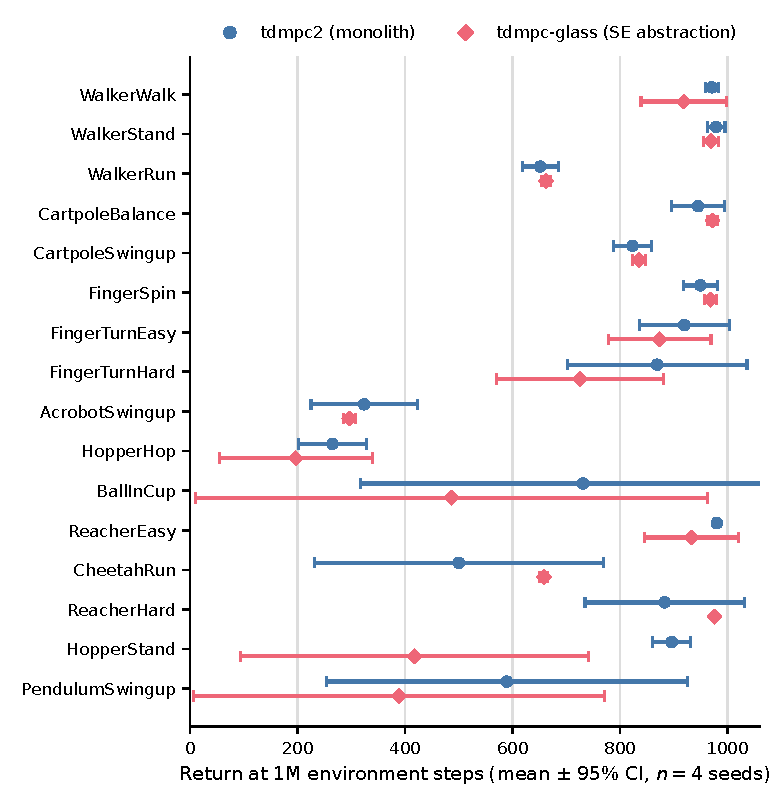
\includegraphics[width=0.72\linewidth]{figures/fig_benchmark_forest.pdf}
\caption{\textbf{Forest plot of the matched 16-task DMC benchmark} (the data of
Table~\ref{tab:bench}): return at 1M environment steps, mean $\pm$ 95\% CI over
$n{=}4$ seeds per arm, tdmpc2 monolith (blue circles) vs.\ tdmpc-glass SE abstraction
(red diamonds), identical code/hyperparameters/harness with the SE objective the only
changed variable. CIs overlap on 15/16 tasks; the single separated case (HopperStand)
favors the monolith and tracks one collapsed glass seed. The SE abstraction buys no
systematic return difference while costing $\sim$1.35$\times$ wall-clock.
Data: \texttt{evidence/dmc\_glass\_vs\_tdmpc2.json}.}
\label{fig:benchforest}
\end{figure}

\paragraph{Findings.}
(1) \emph{No systematic return effect} (Figure~\ref{fig:benchforest}). On 15 of 16 tasks the two tie within overlapping
95\% CIs; the single CI-separated case (HopperStand) favors the monolith and is attributable to a
\emph{single collapsed glass seed}, not a consistent capability gap. The SE objective
produces no systematic gain (nor, at $n{=}4$, a systematic loss). (2) \emph{No systematic stability
difference either.} Both algorithms exhibit occasional seed collapses at this scale (tdmpc2 noisy on
CheetahRun/ReacherHard/BallInCup, glass on HopperStand/Pendulum), so an apparent ``glass is less stable''
read at low $n$ does not survive; the honest statement is high-variance-both-sides at low
seed count. (3) \emph{The one robust difference is cost:} the SE objective adds $\sim$35\%
wall-clock per matched-budget run. The verdict for the monolithic class is therefore the
strongest form of redundancy: \textbf{explicit SE abstraction changes return by nothing detectable
at $n{=}4$ while costing 1.35$\times$ the compute} --- the empirical fingerprint of a basis change
that relocates rather than removes complexity (\S\ref{sec:mechanism}).

\paragraph{A methodological note (why multi-seed was necessary, in both directions).}
A single-seed read of this benchmark would have been misleading \emph{twice over}. On the
high-variance tasks (HopperHop, BallInCup, PendulumSwingup, HopperStand) a single glass run can
look like a ``catastrophic failure'' that the seed spread refutes --- e.g.\ glass HopperHop is
$196{\pm}142$ ($n{=}4$), a variance band, not a capability gap. Symmetrically, at low seed count
tdmpc2 looked uniformly tight and glass uniformly noisy, inviting a ``glass is unstable'' claim that
more seeds refuted (tdmpc2 collapses too --- it is the noisy side on CheetahRun/ReacherHard/BallInCup).
Extreme single measurements invite over-claims in \emph{both}
directions; CI-over-seeds is what separates a result from an artifact --- the same lesson as the
value-decode probe of \S\ref{sec:criterion}, where a single saturated $R^2$ masqueraded as proof.
